\section{The \ourdataset Benchmark}
\label{sec:benchmark}

\subsection{Taxonomy and Scope}
\label{subsec:taxonomy}

\ourdataset covers five core engineering branches (chemical, civil, electrical, industrial, and
mechanical engineering), whose problems are typically solved by quantitative derivations with
checkable intermediate values.
Each branch has three domains, each with two to four areas: 15 domains and 42 areas in all
(\autoref{fig:taxonomy}).
The domains and areas follow the ABET accreditation criteria~\citep{abet2024criteria}, the
curricula of each branch's professional society, and the branch textbooks; we also cross-check the
chemical, electrical, and mechanical lists with four LLMs prompted as curriculum designers.
Domain experts wrote the 150 templates, 30 per branch and ten per domain (8 to 12 in chemical
engineering).
They also assigned each template a level, Easy, Intermediate, or Advanced, by its conceptual
complexity, mathematical sophistication, and procedural depth, so that performance can be compared
across difficulty; the three levels hold 58, 58, and 34 templates.
\autoref{appendix:taxonomy} describes the selection procedure and its prompts, and
\autoref{appendix:sources} lists the textbooks and reference data.

\begin{figure*}[t]
  \centering
  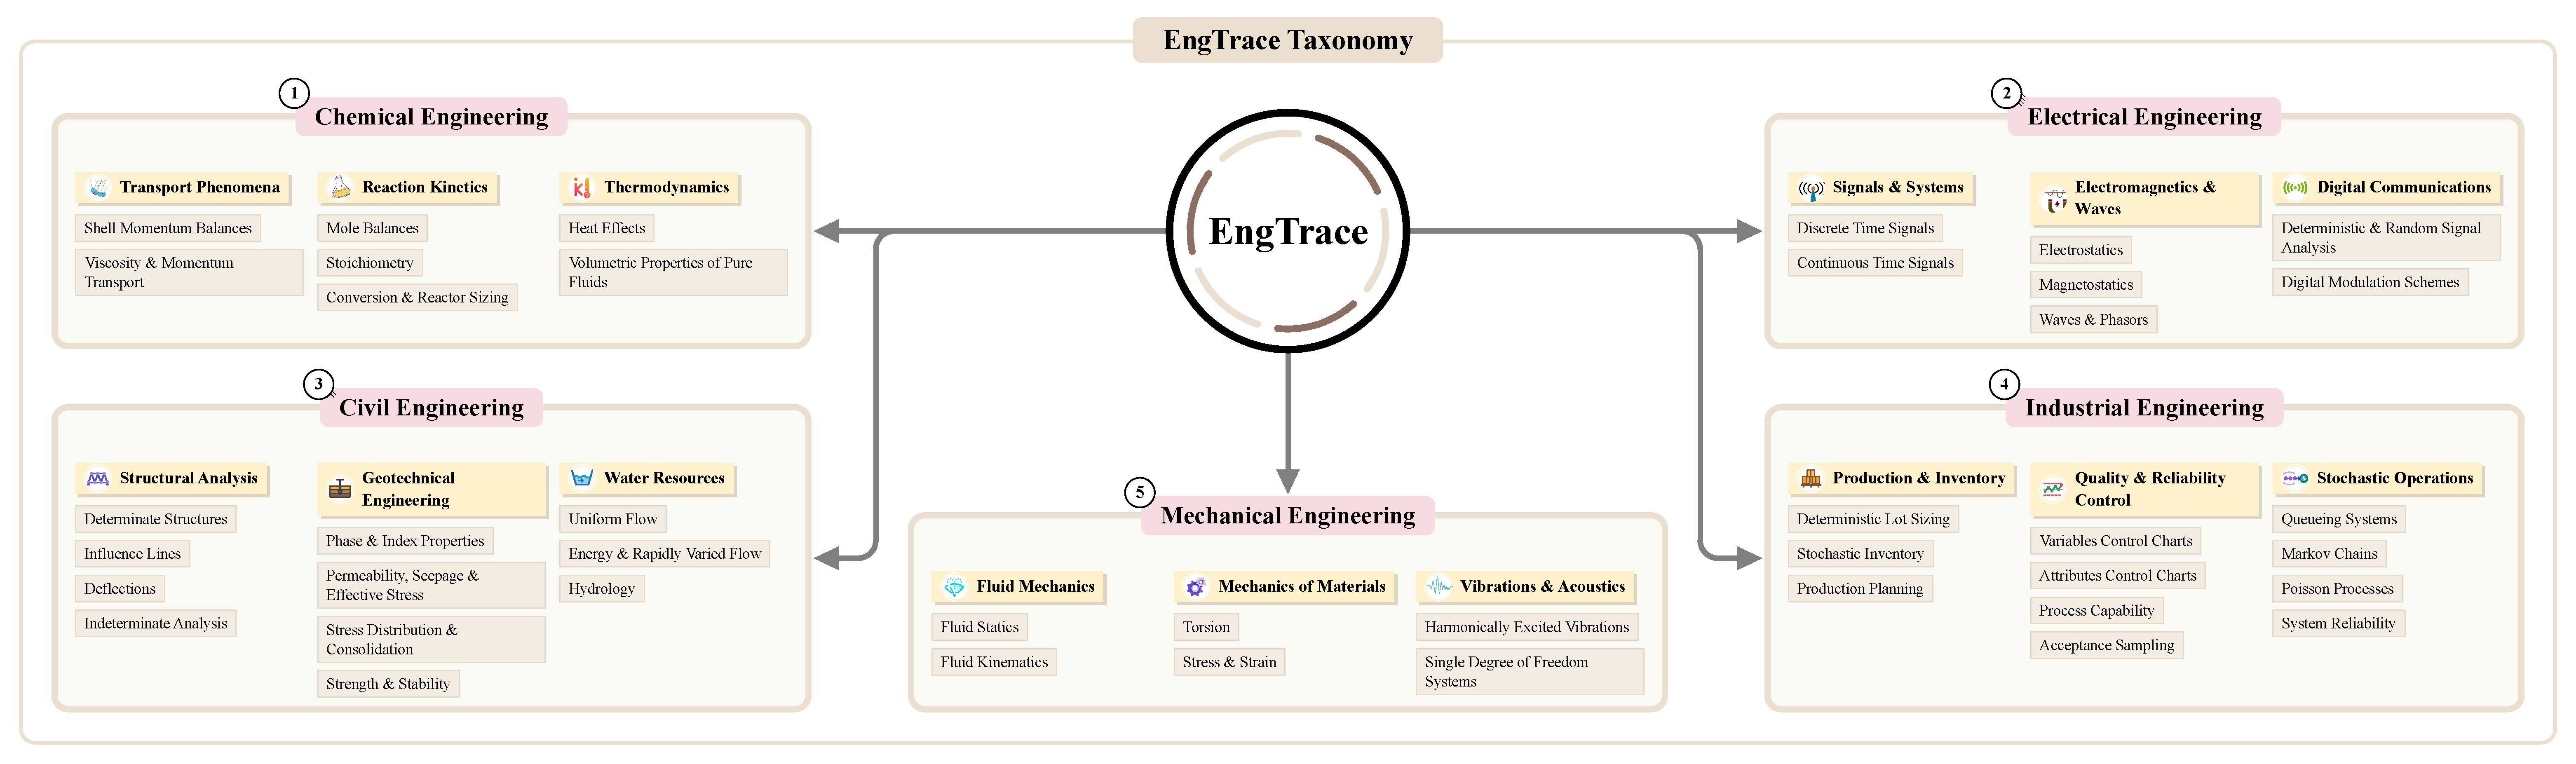
\includegraphics[width=\textwidth]{figs/engtrace-overview-5branch.pdf}
  \caption{The taxonomy of \ourdataset: five engineering branches, each with three domains, and the
    42 areas within the domains.
    Each branch holds 30 templates.}
  \label{fig:taxonomy}
\end{figure*}

\subsection{Templates and Instances}
\label{subsec:templates}

\paragraph{Templates.}
A template is a seeded Python function that generates one problem instance per seed.
It samples physically grounded parameters, with constants and material properties from tables that
record their provenance, and redraws them until the scenario is physically valid (for example, the
flow is laminar or a floating body stays upright).
It then computes every quantity of the solution and writes the question and the gold reasoning
trace, numbered steps that end in the answer.
Because both come from one computation, every intermediate quantity is known exactly, with its
unit; these quantities are the milestones whose coverage we measure (\autoref{sec:evaluation}).
Answers are of six kinds: scalar, vector, array, symbolic, classification, and multipart.

\paragraph{Reasoning paths.}
We call the sequence of equations in a gold trace, with numbers and names masked, the
\emph{reasoning path} of the instance.
In 92 of the 150 templates, the sampled parameters change the reasoning path, for example through a
different governing equation or number of steps; the other 58 templates follow a single path.

\paragraph{Evaluation set.}
We draw 15 instances per template, 2,250 in all, from a private 128-bit seed.
For each template, we pick them round-robin across the reasoning paths and answer forms of its
first 100 draws, skipping repeated questions, so each of the 92 templates with several paths
contributes instances on at least two of them and all 2,250 questions are distinct.
We publish SHA-256 hashes of the instances and of the seed, and will release the seed at
publication so that anyone can verify the instances.
\autoref{appendix:templates} shows template examples and the reasoning-path counts, and
\autoref{appendix:statistics} gives the dataset statistics and the full selection rule.

\subsection{Certification}
\label{subsec:certification}

Because a template error recurs in every instance and gold trace, each template passes three checks
before it enters the benchmark.

\paragraph{Automated integrity checks.}
At 500 seeds per template, far more instances than people can read, automated checks verify that
every printed calculation follows from its printed operands at the printed precision, that
generation is deterministic and keeps its output format, and that every seed generates an instance.
All 150 templates pass, 54 of them after edits.

\paragraph{LLM screen.}
Three LLM judges (Grok 4.6, MiniMax M3, and MiMo-V2.5-Pro), all from families outside the evaluated
models so that no model judges problems it is tested on, score each template's code and three of
its instances for physical plausibility, mathematical correctness, and pedagogical clarity.
After we verify the flags and revise the 24 templates flagged in the first pass, the second pass
rates 147 templates as passing, 3 as controversial (the judges disagree), and none as critically
flawed.
The screen finds problems cheaply but does not decide: it passes 15 templates that a majority of
their experts reject (10.2\% of the 147).

\paragraph{Expert certification.}
Three domain experts from each branch review its 30 templates mixed with four planted defects, one
of each kind: a wrong constant, a wrong unit conversion, a flipped sign, and a printed step that
does not follow from its operands.
Experts know that planted defects exist but not which items they are, and they see neither the
screen's verdicts nor one another's.
For each item, an expert solves one instance by hand before seeing its gold trace, then reviews five
instances, scores the same three criteria, and approves or rejects the template.
Planted defects measure whether experts catch errors; the hand check, whether they work through the
problem.

\paragraph{Outcome.}
Every expert rejects all four planted defects in their branch (60 of 60 readings of the 20
defects), and 459 of 504 hand checks match the template within 1\%; 44 of the 45 mismatches end in
a rejection.
Agreement among the three experts of a branch on approval is 0.914 by Gwet's
AC1~\citep{gwet2008}; Fleiss'~$\kappa$~\citep{fleiss1971} gives 0.589, lower because nearly every
template is approved~\citep{feinstein1990high}.
In the first round, experts cast 43 rejecting verdicts on 22 templates, and in the second, 10 on
five of them; we check each rejection against the instance the expert saw and revise the template
or answer the objection before the same experts review it again.
In the end, all 150 templates are certified by a unanimous vote of their three experts, on code
that still regenerates, byte for byte, the instances they reviewed.
\autoref{appendix:certification} gives the integrity checks, the screening prompt and rubric, the
planted defects, and the counts for each round.
